\section{Implémentation}

\begin{figure}[ht]
  \centering
  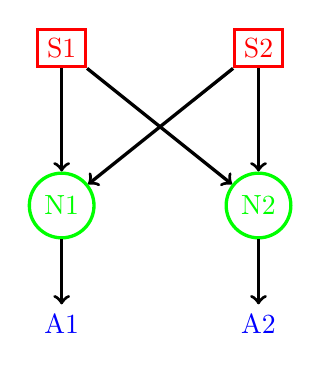
\begin{tikzpicture}[scale=0.5]
 \tikzset{directed/.style={->}} 
  \node[color=blue] (A1) at (0,0) {A1};
  \node[color=blue] (A2) at (5,0) {A2};
  \node[draw, circle, very thick, color=green] (N1) at (0,3) {N1};
  \node[draw, circle, very thick, color=green] (N2) at (5,3) {N2};
  \node[draw, very thick, color=red] (S1) at (0,7) {S1};
  \node[draw, very thick, color=red] (S2) at (5,7) {S2};
  \draw[very thick, directed] (S1) -- (N1);
  \draw[very thick, directed] (S2) -- (N1);
  \draw[very thick, directed] (S1) -- (N2);
  \draw[very thick, directed] (S2) -- (N2);
  \draw[very thick, directed] (N1) -- (A1);
  \draw[very thick, directed] (N2) -- (A2);
\end{tikzpicture}

  \caption{Réseau de neurone à deux neurones}
  \label{graphInit}
\end{figure}

\paragraph{}
Nous pouvons voir sur le schéma \ref{graphInit} que trois types d'objets sont
présents dans notre conception d'un réseau de neurones:\\
\begin{description}
  \item[Les stimuli] Réalisés en rouge sur le schéma, ils génèrent les signaux
    qui activent les premiers neurones et ainsi active le réseau.
  \item[Les actions] Affichés en bleu sur le schéma, elles sont les sorties de
    notre système, elles correspondent à la décision effectué par notre réseau.
  \item[Les neurones] Cœur même du réseau, ils sont là pour effectuer la prise
    de décision en fonction des entrées qu'ils possèdent.
\end{description}

\paragraph{}
Ces trois éléments sont donc la base de notre réseau, cependant nous avons
décidé de rendre générique notre réseau et ainsi notre réseau stockera une liste
de stimuli et de réactions.

\paragraph{}
Il a ensuite fallu déterminer la façon de parcourir tous les neurones pour les
mettre à jour. Cette réflexion a fait émerger diverses techniques cependant deux
avaient un effet similaire avec une base commune (les stimuli sont le départ du
calcul du réseau) mais modifiaient la façon de considérer chaque
neurone:\\

\begin{enumerate}
  \item La première consistait à considérer que chaque neurone connait les
    neurones qui lui envoient un signal. Il peut donc les interroger, obtenant
    ainsi les informations nécessaires au calcul de sa sortie.
  \item La seconde considérait que chaque neurone avait connaissance des neurones
    concernés par sa sortie, il pouvait donc leur signaler qu'une valeur avait
    été mise à jour.
\end{enumerate}

La seconde solution était bloquante pour l'apprentissage, étant donné que les
poids stockés par le neurone concernaient les autres neurone, il nécessitait
donc un lien autre que ceux acceptés par le standard de neurone.

Cela a donc mis en évidence l'impossibilité de cette méthode, elle a donc été
naturellement écarté.

\paragraph{}


\paragraph{}
Ne souhaitant pas attribuer aux neurones des caractéristiques qui ne leur étaient
pas nécessaires, nous nous sommes demandé ce qui était intrinsèque au
fonctionnement de l'entité et ce qui relevait de la particularité de notre
réseau.

\paragraph{}
Après réflexion nous sommes arrivé à déterminer comme cœur du neurone, les
parties suivantes:\\

\begin{description}
  \item[Nom] Chaque neurone est doté d'un nom qui permettra de le distinguer
    lors de l'envoi de chaque valeur vers les neurones concernés
  \item[Poids] Chaque neurone va pondérer chacune de ses entrées en fonction
    d'un dictionnaire contenant le poids attribué à chaque neurone voisine
  \item[Output] Liste des neurones de sortie pour permettre à la fin de chaque
    calcul, d'activer ces derniers qui vont tenter de calculer leur propre
    sortie
\end{description}

Il est apparu après le début de la phase d'implémentation qu'il était nécessaire
de rajouter certaines variables, pour ne pas activer un neurone qui n'aurait pas
toute ses valeurs en entrée active.
Pour cela nous avons du rajouter deux variables:\\

\begin{description}
  \item[Somme] Cette valeur accumule la somme des entrées depuis la dernière
    activation totale, c'est à dire qu'à chaque appel de la part des neurones
    précédents, elle va rajouter la valeur en entrée pondéré dans sa valeur
    globale et va ensuite la déchargé lors de son actualisation personnelle. 
  \item[Nombre d'entrée manquante] Il est facile de connaître le nombre d'entrée
    totale grâce au dictionnaire des poids qui va nous donner par sa taille, ce
    nombre, cependant il est nécessaire de savoir si toute les valeurs en entrée
    attendues sont disponibles ou pas. Si oui, alors le neurone calcule sa
    sortie et envoi sa sortie aux neurones connectés.
  \end{description}
